%%%%%%%%%%%%%%%%%%%%%%%%%%%%%%%%%%%%%%%%%%%%%%%%%%%%%%%%%%%%%%%%%%%%%%%%%%%%%%%%
%%%%%%%%%%%%%%%%%%   Vorlage für eine Abschlussarbeit   %%%%%%%%%%%%%%%%%%%%%%%%
%%%%%%%%%%%%%%%%%%%%%%%%%%%%%%%%%%%%%%%%%%%%%%%%%%%%%%%%%%%%%%%%%%%%%%%%%%%%%%%%

% Erstellt von Maximilian Nöthe, <maximilian.noethe@tu-dortmund.de>
% ausgelegt für lualatex und Biblatex mit biber

% Kompilieren mit
% latexmk --lualatex --output-directory=build thesis.tex
% oder einfach mit:
% make

\documentclass[
  tucolor,       % remove for less green,
  BCOR=12mm,     % 12mm binding corrections, adjust to fit your binding
  parskip=half,  % new paragraphs start with half line vertical space
  open=any,      % chapters start on both odd and even pages
  cleardoublepage=plain,  % no header/footer on blank pages
]{tudothesis}


% Warning, if another latex run is needed
\usepackage[aux]{rerunfilecheck}

% just list chapters and sections in the toc, not subsections or smaller
\setcounter{tocdepth}{1}

%------------------------------------------------------------------------------
%------------------------------ Fonts, Unicode, Language ----------------------
%------------------------------------------------------------------------------
\usepackage{fontspec}
\defaultfontfeatures{Ligatures=TeX}  % -- becomes en-dash etc.

% load english (for abstract) and ngerman language
% the main language has to come last
\usepackage[american, ngerman]{babel}

% intelligent quotation marks, language and nesting sensitive
\usepackage[autostyle]{csquotes}

% microtypographical features, makes the text look nicer on the small scale
\usepackage{microtype}

%------------------------------------------------------------------------------
%------------------------ Math Packages and settings --------------------------
%------------------------------------------------------------------------------

\usepackage{amsmath}
\usepackage{amssymb}
\usepackage{mathtools}

% Enable Unicode-Math and follow the ISO-Standards for typesetting math
\usepackage[
  math-style=ISO,
  bold-style=ISO,
  sans-style=italic,
  nabla=upright,
  partial=upright,
  warnings-off={mathtools-colon,mathtools-overbracket}, % suppress some unnecessary warnings
]{unicode-math}
\setmathfont{Latin Modern Math}

% nice, small fracs for the text with \sfrac{}{}
\usepackage{xfrac}


%------------------------------------------------------------------------------
%---------------------------- Numbers and Units -------------------------------
%------------------------------------------------------------------------------

\usepackage[
  locale=DE,
  separate-uncertainty=true,
  per-mode=symbol-or-fraction,
]{siunitx}

%------------------------------------------------------------------------------
%-------------------------------- tables  -------------------------------------
%------------------------------------------------------------------------------

\usepackage{booktabs}       % \toprule, \midrule, \bottomrule, etc

%------------------------------------------------------------------------------
%-------------------------------- graphics -------------------------------------
%------------------------------------------------------------------------------

\usepackage{graphicx}
% currently broken
% \usepackage{grffile}

% allow figures to be placed in the running text by default:
\usepackage{scrhack}
\usepackage{float}
\floatplacement{figure}{htbp}
\floatplacement{table}{htbp}

% keep figures and tables in the section
\usepackage[section, below]{placeins}

% allows to include PDFs as full pages
\usepackage{pdfpages}

% Set the PDF Version of this document to 1.7 (1.4 is the current default)
% This is needed so that PDFs with Version >1.5 can be included
\pdfvariable minorversion=7

%------------------------------------------------------------------------------
%---------------------- customize list environments ---------------------------
%------------------------------------------------------------------------------

\usepackage{enumitem}

%------------------------------------------------------------------------------
%------------------------------ Bibliographie ---------------------------------
%------------------------------------------------------------------------------

\usepackage[
  backend=biber,   % use modern biber backend
  autolang=hyphen, % load hyphenation rules for if language of bibentry is not
                   % german, has to be loaded with \setotherlanguages
                   % in the references.bib use langid={en} for english sources
]{biblatex}
\addbibresource{references.bib}  % the bib file to use
\DefineBibliographyStrings{german}{andothers = {{et\,al\adddot}}}  % replace u.a. with et al.


% Last packages, do not change order or insert new packages after these ones
\usepackage[pdfusetitle, unicode, linkbordercolor=tugreen, citebordercolor=tugreen]{hyperref}
\usepackage{bookmark}
\usepackage[shortcuts]{extdash}

%------------------------------------------------------------------------------
%-------------------------    Angaben zur Arbeit   ----------------------------
%------------------------------------------------------------------------------

\author{Jonas Ollesch}
\title{Grenzen auf Majoron-Neutrino-Kopplungen aus Supernovaexplosionen in verschiedenen Basen}
\date{2023}
\birthplace{Recklinghausen}
\chair{Lehrstuhl für Theoretische Teilchenphysik}
\division{Fakultät Physik}
\thesisclass{Bachelor of Science}
\submissiondate{14. Juli 2023}
\firstcorrector{Prof. Dr. Heinrich Päs}
\secondcorrector{Jun-Prof. Dr. Emmanuel Stamou}

% tu logo on top of the titlepage
\titlehead{
\includegraphics[height=1.5cm]{logos/tu-logo.pdf}}

\begin{document}
\frontmatter
\maketitle

% Gutachterseite
\makecorrectorpage

% hier beginnt der Vorspann, nummeriert in römischen Zahlen
\thispagestyle{plain}

\section*{Kurzfassung}
In dieser Arbeit betrachten wir die Kopplung zwischen Neutrinos als Majoranateilchen, also Teilchen, die mit ihren Antiteilchen übereinstimmen, und Majoronen, den Teilchen, die,
ähnlich wie das Higgs-Boson für alle anderen Teilchen, Neutrinos ihre Masse verleihen.
Über den hypothetischen neutrinolosen Doppelbetazerfall und Beobachtungen der Spektren und Luminositäten von Supernovae lassen die die zulässigen Kopplungparameterbereiche limitieren.
Es gelingt uns, mithilfe beobachteter Daten der Supernova SN1987A, die Kopplungsparameter $|g_{i j}|$ auf $|g_{i j}| < \frac{\num{0.83} \cdot 10^{-8}}{m_J} \,\si{\mega\eV}$ 
in einem Bereich von $\SI{100}{\eV} < m_J < \SI{100}{\mega\eV}$ einzuschränken.
Gemeinsam mit der Neutrinomassengrenze von $m_1 < \SI{0.8}{\eV}$ aus dem KATRIN-Experiment und der Einschränkung $g_1 < 10^{-4}$ aus einer Betrachtung der Neutrinospektren lässt sich der in \autoref{fig:exclusionregionfinal}
dargestellte Parameterbereich ausschließen. \\
Nach abschließendem Vergleich mit den von Hau Zhang in \cite{hauhau} aus dem neutrinolosen Doppelbetazerfall erhaltenen Obergrenzen auf die Kopplung $g_{ee}$ mit $\num{0.4} \, \cdot \, 10^{-5} < g_{ee} < \num{0.9} \, \cdot \, 10^{-5}$ sehen wir, dass
der Doppelbetazerfall die von uns ermittelte Ausschlussregion nicht weiter einschränkt.

\section*{Abstract}
\begin{foreignlanguage}{english}
In this thesis, we discuss the coupling between neutrinos as majorana particles, thus particles that coincide with their anti particles, and majorons, the particles that, like the Higgs boson does for all other
particles, give the neutrios their mass.
The valid coupling parameter regions can be limited by discussing the hypothetical neutrinoless double beta decay and observed supernova spectra and their luminosities.
We succeed in limiting the coupling parameters $|g_{i j}|$ to $|g_{i j}| < \frac{0.83 \cdot 10^{-8}}{m_J} \,\si{\mega\eV}$ in a range of $\SI{100}{\eV} < m_J < \SI{100}{\mega\eV}$.
Together with the neutrino mass limit of $m_1 < 0.8 \,\si{\eV}$, obtained from the KATRIN experiment, and the restriction $g_1 < 10^{-4}$ from neutrino spectra, we gain the exclusion region represented in
\autoref{fig:exclusionregionfinal}. \\
By comparing our results to the upper limits on $g_{ee}$ from neutrinoless double beta decay, obtained by Hau Zhang in \cite{hauhau} with $\num{0.4} \, \cdot \, 10^{-5} < g_{ee} < \num{0.9} \, \cdot \, 10^{-5}$, we see no further
modification of the assumed exclusion region.
\end{foreignlanguage}

\tableofcontents

\mainmatter
% Hier beginnt der Inhalt mit Seite 1 in arabischen Ziffern
\chapter{Einleitung}
\label{chap:einleitung}

Neutrinos sind nach dem Standardmodell der Teilchenphysik neutrale, masselose Leptonen, die nur über die schwache Wechselwirkung an andere Elementarteilchen koppeln.
In zwei unabhängigen Experimenten konnten von Arthur McDonald Takaaki Kajita allerdings bewiesen werden, dass der lange vorhergesagte Prozess der Neutrinooszillationen tatsächlich existiert.
Diese Neutrinooszillation, also das zeitlich und räumlich periodische Wechseln des Neutrinoflavours, setzt allerdings eine endliche Ruhemasse voraus.
Damit können Neutrinos nicht, wie vom Standardmodell angenommen, masselos sein.

Das Standardmodell muss also um neue Physik ergänzt werden, um die Neutrinomasse zu berücksichtigen.
Eine Möglichkeit, die endliche, aber, verglichen mit den anderen Leptonen verschwindend geringe Masse zu erklären, ist, Neutrinos als Majoranateilchen einzuführen.
Majoranateilchen beschreiben Teilchen, die mit ihren Antiteilchen übereinstimmen.
Im Falle der Neutrinos müsste so die jedem Lepton zugeordnete Leptonzahl, die bei allen bisher beobachteten Prozess eine Erhaltungsgröße darstellt, spontan gebrochen sein.
Diese spontane Symmetriebrechung führen wir später durch das Majoronenfeld ein, das linkshändige Neutrinos mit rechtshändigen Antineutrinos und umgekehrt verknüpft.
Es besitzt die Majoronen, sogenannte Goldstone-Bosonen, als Botenteilchen. \\
Um diese Majoronen zu finden, werden konkret zwei Prozesse näher betrachtet.
Der neutrinolose Doppelbetazerfall, bei dem zwei Neutronen in einem Atomkern gleichzeitig unter möglicher Emission eines Majorons in zwei Protonen und Elektronen zerfallen und Supernovaexplosionen, bei denen
Majoronen die Kühlung und die Neutrinospektren beeinflussen könnten. \\
Hier legen wir den Fokus auf den Prozess der Supernovae.
Anhand verschiedener Basen werden wir uns die Propagation von Neutrinos in dichten Medien deutlich machen und konkret beleuchten, 
inwiefern Eigenzustände der Massenbasis und der Materiebasis miteinander verknüpft sind.
Durch Betrachtung verschiedener Argumente und aufgenommener Daten der Supernova SN1987A wird es uns so gelingen, Grenzen auf die Neutrinomasse und Kopplungen zwischen Majoronen und Neutrinos zu erhalten.
Haben wir diese Grenzen erhalten, stellen wir die Ergebnisse analog zu \cite{päspaper} grafisch dar, um ein anschauliches Bild für die entstehenden Ausschlussregionen zu erhalten und ziehen abschließend einen Vergleich
zu den von Hau Zhang in \cite{hauhau} erzielten Ergebnissen des Doppelbetazerfalls.



\chapter{Struktur der Arbeit}

Eine mögliche Struktur der Arbeit sieht wie folgt aus:

\begin{enumerate}
    \item \textbf{Einleitung}\\
        In der \emph{kurzen} Einleitung wird die Motivation für die Arbeit
        dargestellt und ein Einblick in die kommenden Kapitel gegeben.
    \item \textbf{Theoretische Grundlagen}\\
        Alles was an theoretischen Grundlagen benötigt wird, sollte auch eher kurz gehalten werden.
        Statt Grundlagenwissen zu präsentieren, eher auf die entsprechenden Lehrbücher verweisen.
        Etwa: Tiefer gehende Informationen zur klassischen Mechanik entnehmen Sie bitte \cite{kuypers}.
    \item \textbf{Ergebnisse} \\
        Der eigentliche Teil der Arbeit, das was getan wurde.
    \item \textbf{Zusammenfassung und Ausblick} \\
        Zusammenfassung der Ergebnisse, Optimierungsmöglichkeiten, mögliche weitergehende Untersuchungen.
\end{enumerate}

Die Gliederung sollte auf der einen Seite nicht zu fein sein, auf der anderen Seite
sollten sich klar unterscheidende Abschnitte auch kenntlich gemacht werden.

In der hier verwendeten \KOMAScript-Klasse \texttt{scrbook} ist die oberste Gliederungsebene,
die in der Bachelorarbeit verwendet werden sollte, das \texttt{\textbackslash chapter}.

Ein Kapitel sollte erst dann in tiefere Gliederungsebenen unterteilt werden, wenn es auch wirklich etwas zu unterteilen gibt. Es sollte keine Kapitel mit nur einem Unterkapitel (\texttt{\textbackslash section}) geben.

In dieser Vorlage ist die Tiefe des Inhaltsverzeichnisses auf \texttt{chapter} und \texttt{section} beschränkt. Möchten Sie diese Beschränkung aufheben, entfernen Sie den Befehl
\begin{verbatim}
            \setcounter{tocdepth}{1}
\end{verbatim}
aus der Präambel oder ändern Sie den Zahlenwert entsprechend. Das Inhaltsverzeichnis sollte für eine Bachelorarbeit auf eine Seite passen.

\chapter{Theoretische Grundlagen}

\section{Neutrinos im Standardmodell}



\section{Spontane Symmetriebrechung}

\section{Neutrinos in verschiedenen Basen}

\section{Einfluss von Majoronen auf Supernovaexplosionen}


\chapter{Abbildungen und Tabellen}

\section{Abbildungen}

Achten Sie bei ihren Plots auf ausreichend große Achsenbschriftungen, ausreichende Schriftdicken und gut unterscheidbare Farben.
Im Idealfall haben Sie im Plot und der Arbeit die gleiche Schriftgröße und Schriftart.
Dies lässt sich durch Erstellen des Plots in der korrekten Größe und Einbinden mit dem optionalen Argument \texttt{scale=1} erreichen. Ein Beispiel sehen Sie in Abbildung \ref{fig:bsp}.

Nutzen Sie wenn möglich Vektorgrafiken (pdf) und nur in Ausnahmen Rastergrafiken wie .png oder .jpg.
Setzen Sie Punkte hinter Abbildungsunterschriften.

\begin{figure}
    \centering
    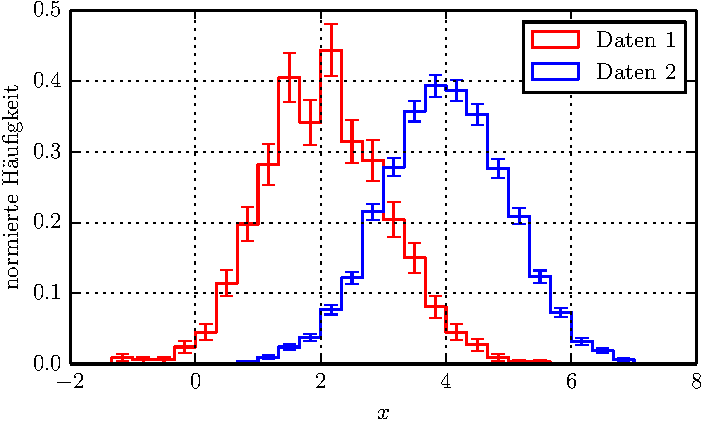
\includegraphics[scale=1]{./Plots/Histogramm.pdf}
    \caption{Ein Histogramm mit Fehlerbalken für zwei Datensätze, Schriftgröße und -art entsprechen der des Dokuments.}
    \label{fig:bsp}
\end{figure}

\section{Tabellen}

Tabellen sollten so einfach wie möglich aufgebaut sein, verzichten Sie auf zu viele Linien. In fast allen Fällen reichen drei horizontale Linien aus, jeweils über und unter der Tabelle und zwischen den Spaltenüberschriften und der eigentlichen Tabelle.

Das Paket \texttt{booktabs} stellt hierfür \verb_\toprule_, \verb_\midrule_ und 
\verb_\bottomrule_ zur Verfügung.
Das Paket \texttt{siunitx} stellt eine extrem mächtige neue Spalteneinstellung bereit: \texttt{S}, mit ihr können Zahlen und Einheiten sehr sauber und gut ausgerichtet gesetzt werden.

Diese Vorlage geht von Tabellenüberschriften aus, möchten Sie dagegen Tabellenunterschriften entfernen Sie das entsprechende optionale Argument für die Dokumentenklasse in der Präambel.

Ein Beispiel ist Tabelle~\ref{tab:bsp}.
\begin{table}
    \centering
    \caption{Beispieltabelle mit willkürlichen Werten, für die Zahlenwerte wurde die S-Option aus \texttt{siunitx} verwendet.}
    \label{tab:bsp}
    \begin{tabular}{S[table-format=4.2] S[table-format=3.2]}
        \toprule
        {$p \mathrel{/} \si{\pascal}$}  & {$T \mathrel{/} \si{\kelvin}$} \\
        \midrule
        1024,23 & 273,15 \\
        1025,31 & 274,5 \\
        1026,27 & 276,2 \\
        \bottomrule
    \end{tabular}
\end{table}


\appendix
% Hier beginnt der Anhang, nummeriert in lateinischen Buchstaben
\chapter{Anhang}

\backmatter
\printbibliography

\cleardoublepage
% From https://www.tu-dortmund.de/studierende/im-studium/pruefungsangelegenheiten/allgemeine-vordrucke/
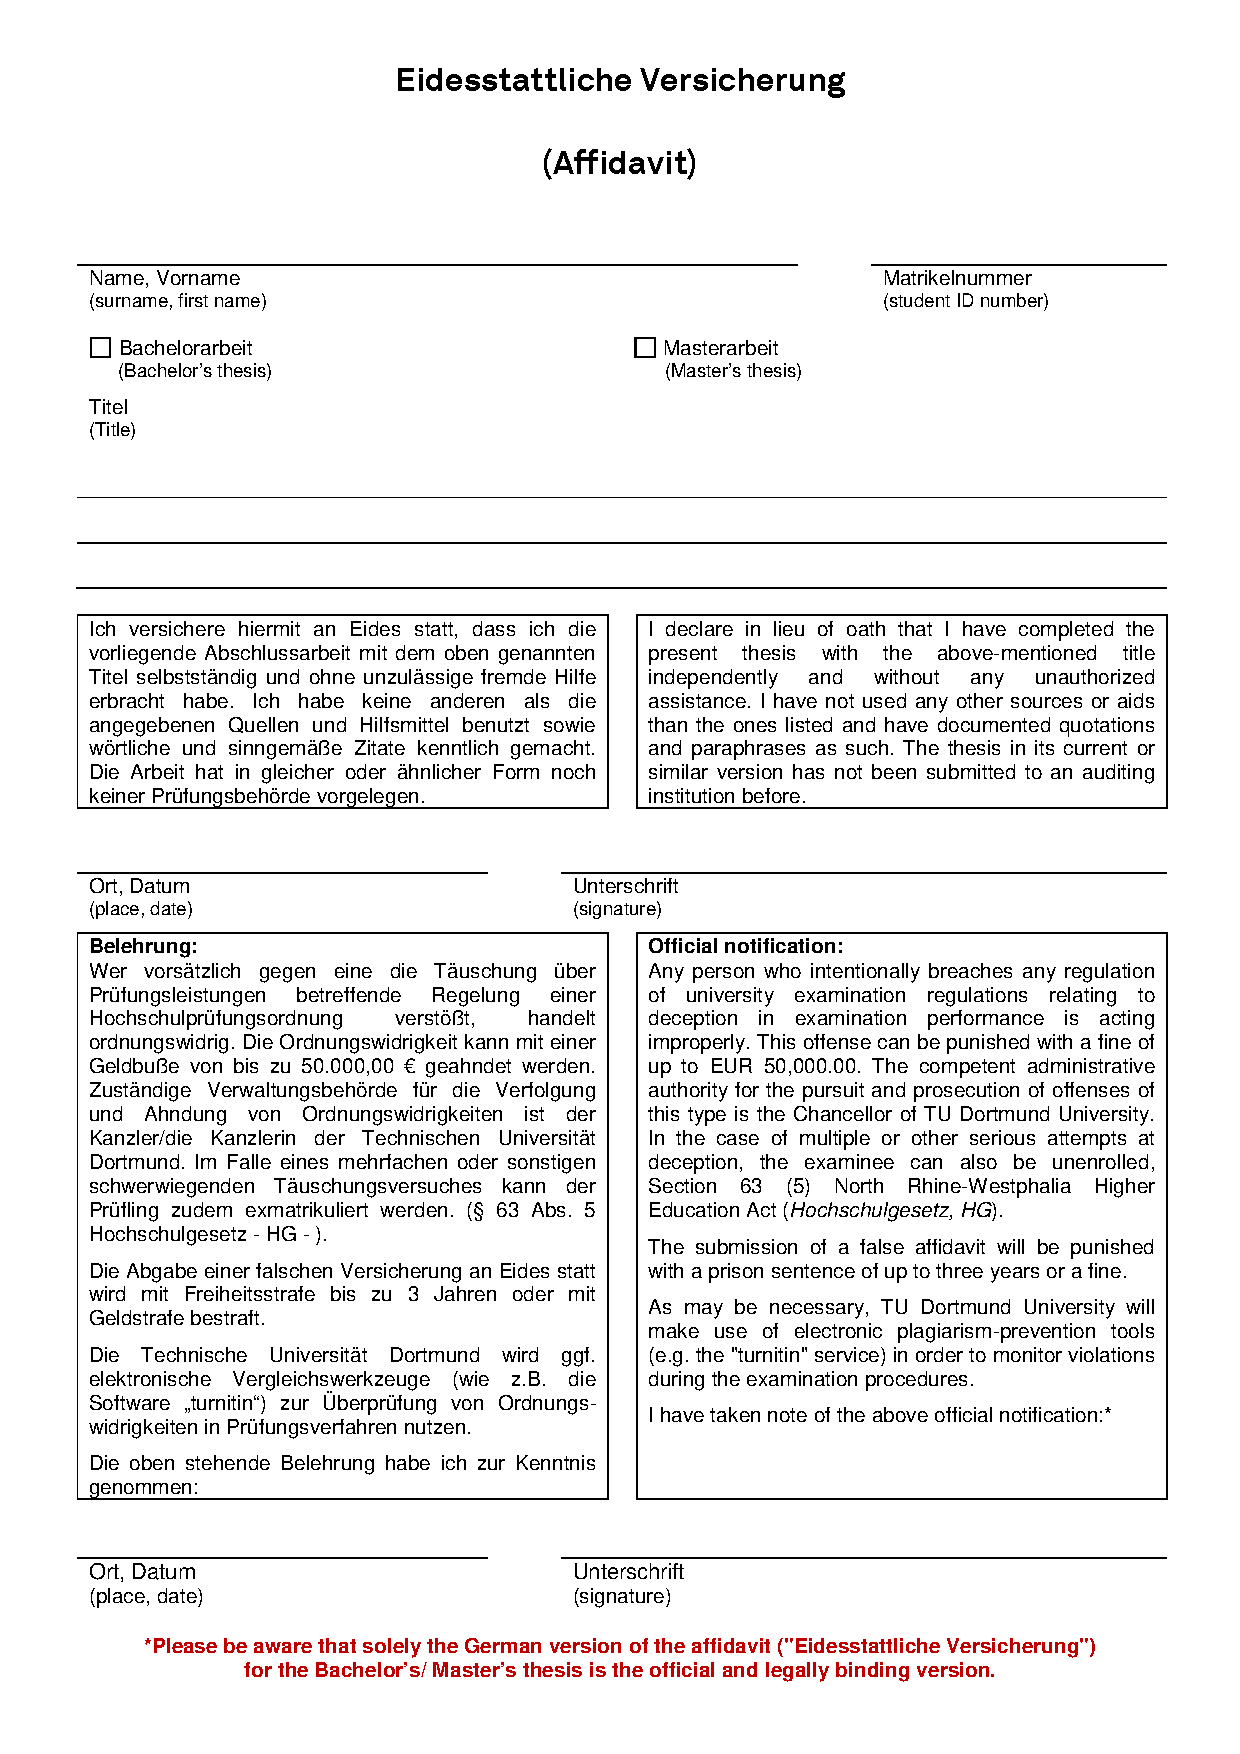
\includepdf{content/Eidesstattliche_Versicherung.pdf}

\end{document}
